\documentclass[pdf]{beamer}

\usepackage{graphicx}
\usepackage{tikz}
\usepackage{amsmath}
\usetikzlibrary{mindmap,trees,shapes.symbols,shadows,decorations.pathmorphing,shapes,decorations.text,arrows}
\usepackage{verbatim}
\DeclareMathOperator*{\argmin}{\arg\!\min}

\mode<presentation>{}
\usetheme{CambridgeUS}
\usecolortheme{beaver}
\useinnertheme{rounded}

\title[Quantile Regression]{Quantile Regression\\Reference range of Thyroid function test in pregnancy}
\author{Kevin Brosnan}
\institute[UL]{University of Limerick}
\date{$13^{th}$ October, 2015}

\usebackgroundtemplate{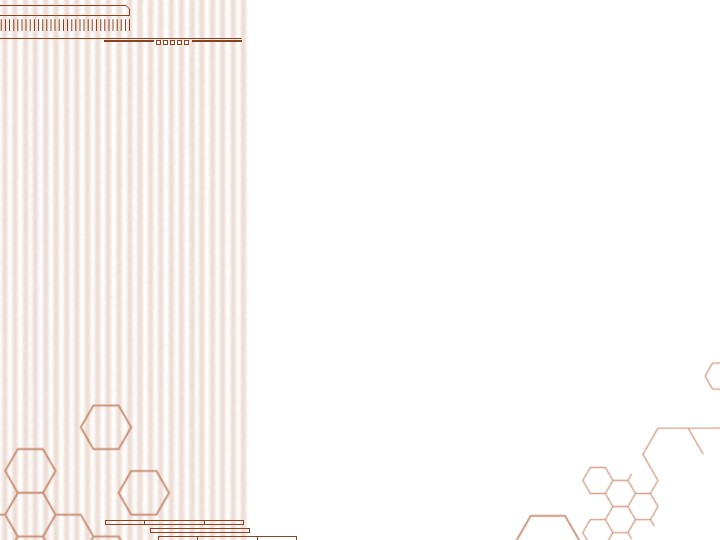
\includegraphics[width=13cm]{TitlepageBackground.jpg}}
\beamertemplatenavigationsymbolsempty

\begin{document}

\begin{frame}[plain]
    \titlepage
\end{frame}

\usebackgroundtemplate{}

\section{Table of Contents}
\begin{frame}
\begin{figure}
    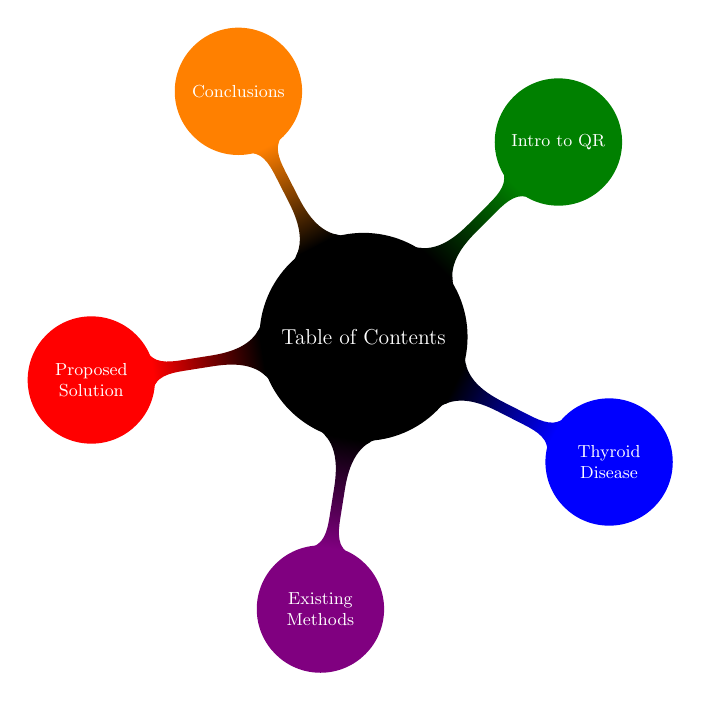
\begin{tikzpicture}[scale=0.7]
        \path[mindmap,concept color=black,text=white]
            node[concept,scale=0.65] {Table of Contents}
            [clockwise from=45]
                child[concept color=green!50!black, grow=45] {node[concept,scale=0.7] {Intro to QR}}
                child[concept color=blue, grow=-27] {node[concept,scale=0.7] {Thyroid Disease}}
                child[concept color=violet, grow=-99] {node[concept,scale=0.7] {Existing Methods} }
                child[concept color=red, grow=-171] {node[concept,scale=0.7] {Proposed Solution}}
                child[concept color=orange, grow=117] {node[concept,scale=0.7] {Conclusions} }
                ;
    \end{tikzpicture}
\end{figure}
\end{frame}

\section{Intro to QR} % Chapter 2
\begin{frame}
\begin{figure}
    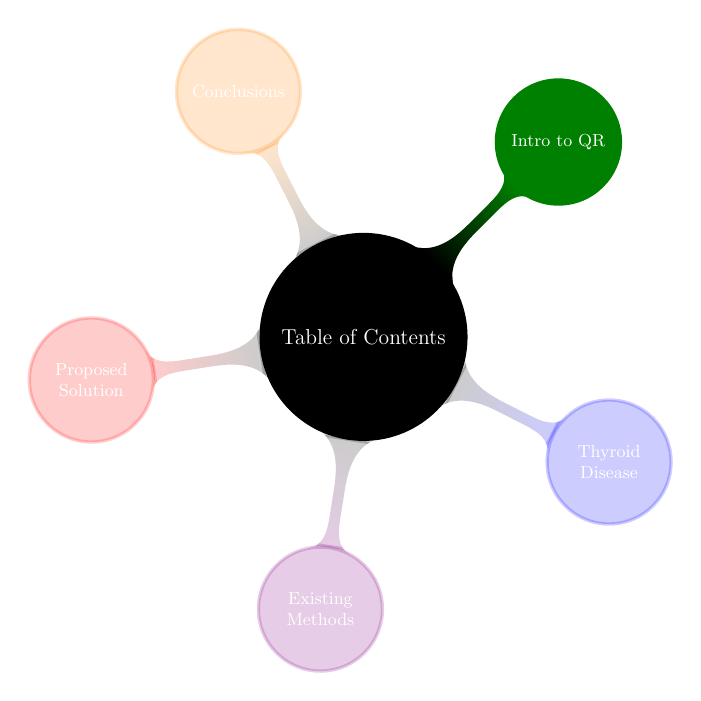
\begin{tikzpicture}[scale=0.7]
        \path[mindmap,concept color=black,text=white]
            node[concept,scale=0.65] {Table of Contents}
            [clockwise from=45]
                child[concept color=green!50!black, grow=45] {node[concept,scale=0.7] {Intro to QR}}
                child[concept color=blue,opacity=0.2, grow=-27] {node[concept,scale=0.7,opacity=0.2,text opacity=1] {Thyroid Disease}}
                child[concept color=violet,opacity=0.2, grow=-99] {node[concept,scale=0.7,opacity=0.2,text opacity=1] {Existing Methods} }
                child[concept color=red,opacity=0.2, grow=-171] {node[concept,scale=0.7,opacity=0.2,text opacity=1] {Proposed Solution}}
                child[concept color=orange,opacity=0.2, grow=117] {node[concept,scale=0.7,opacity=0.2,text opacity=1] {Conclusions} }
                ;
    \end{tikzpicture}
\end{figure}
\end{frame}

\begin{frame}
\only<1>{
\center{\textbf{Interested in understanding the \underline{entire} distribution of the data}}
\begin{figure}
    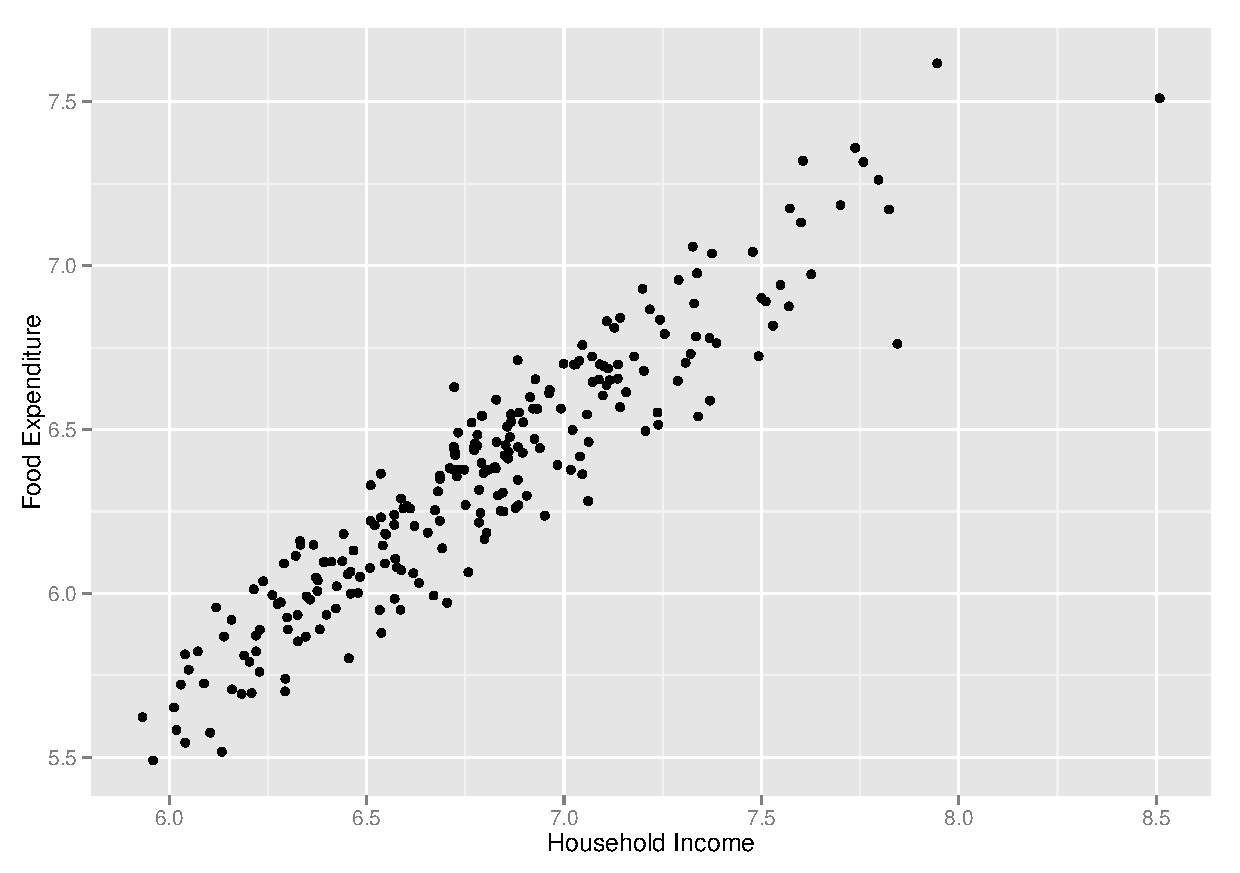
\includegraphics[width=10.5cm]{IntroToQR1.pdf}
\end{figure}
}

\only<2>{
\center{\textbf{What does this \underline{actually} tell us?}}
\begin{figure}
    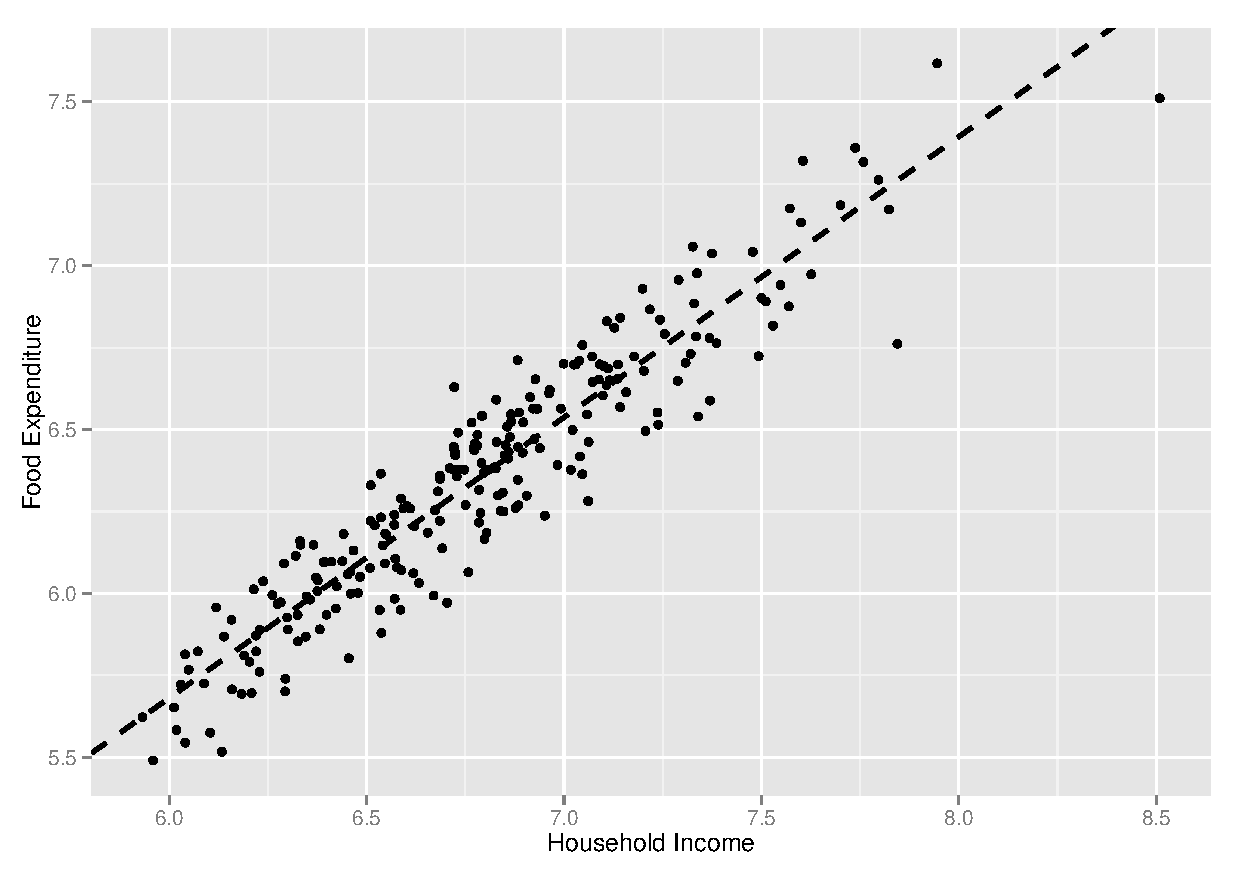
\includegraphics[width=10.5cm]{IntroToQR2.pdf}
\end{figure}
}

\only<3>{
\center{\textbf{Quantile Regression helps to \underline{complete} the picture}}
\begin{figure}
    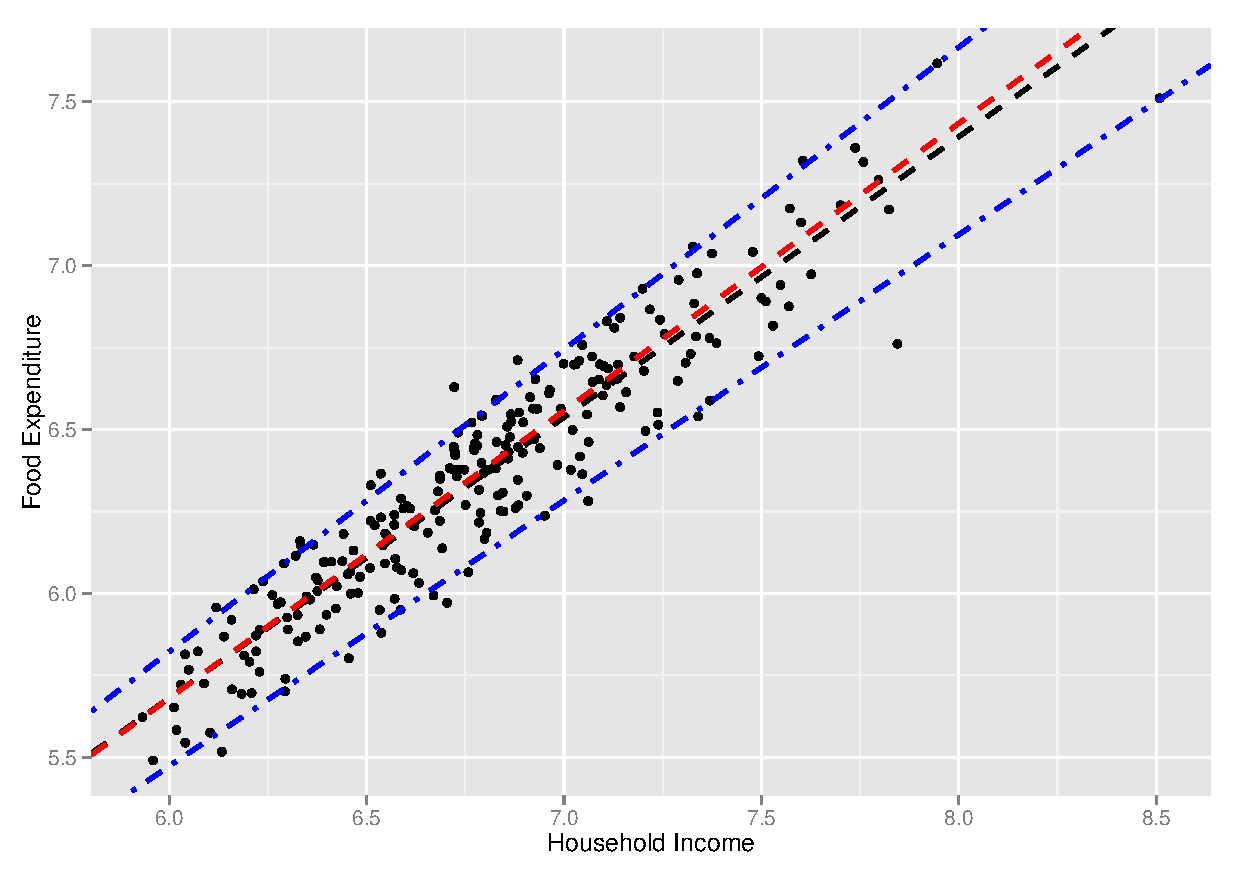
\includegraphics[width=10.5cm]{IntroToQR3.pdf}
\end{figure}
}
\end{frame}

\section{Thyroid Disease} % First half of Chapter 3
\begin{frame}
\begin{figure}
    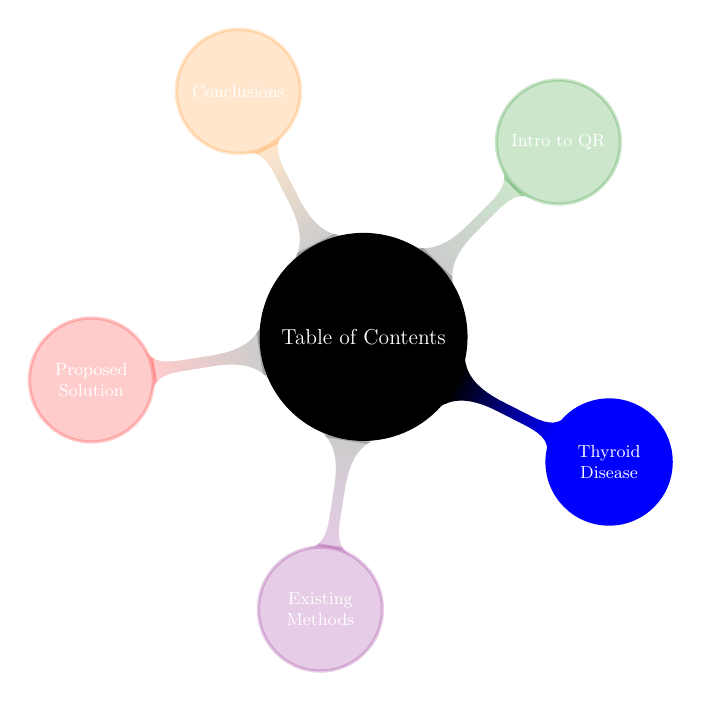
\begin{tikzpicture}[scale=0.7]
        \path[mindmap,concept color=black,text=white]
            node[concept,scale=0.65] {Table of Contents}
            [clockwise from=45]
                child[concept color=green!50!black,opacity=0.2, grow=45] {node[concept,scale=0.7,opacity=0.2,text opacity=1] {Intro to QR}}
                child[concept color=blue,grow=-27] {node[concept,scale=0.7] {Thyroid Disease}}
                child[concept color=violet,opacity=0.2, grow=-99] {node[concept,scale=0.7,opacity=0.2,text opacity=1] {Existing Methods} }
                child[concept color=red,opacity=0.2, grow=-171] {node[concept,scale=0.7,opacity=0.2,text opacity=1] {Proposed Solution}}
                child[concept color=orange,opacity=0.2, grow=117] {node[concept,scale=0.7,opacity=0.2,text opacity=1] {Conclusions} }
                ;
    \end{tikzpicture}
\end{figure}
\end{frame}

\begin{frame}
\only<1>{
    \begin{figure}[width=\paperwidth, height=\paperheight]
    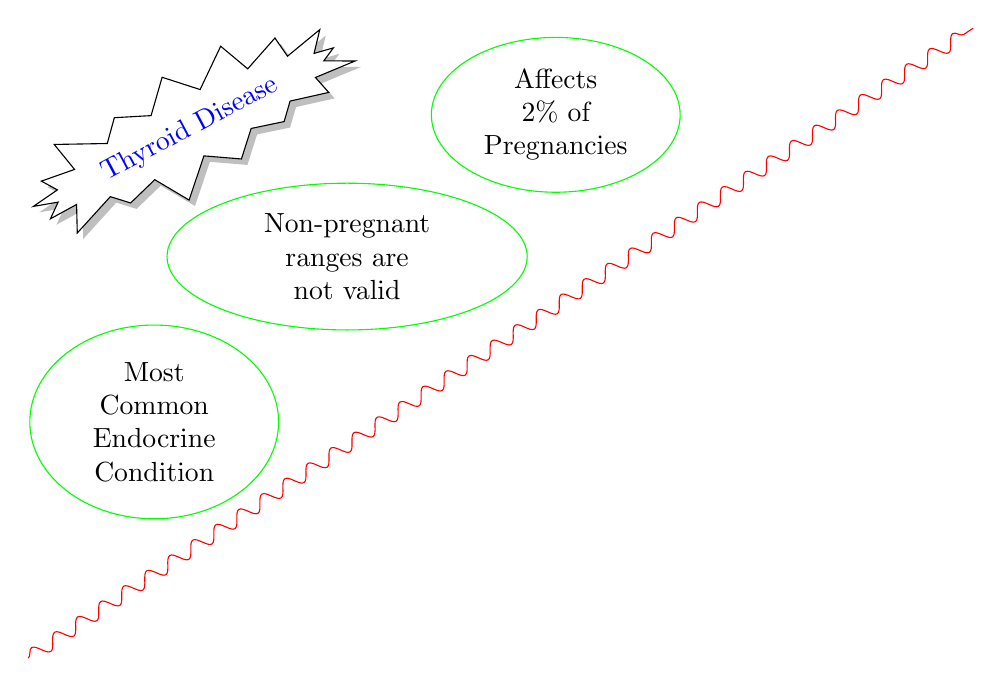
\begin{tikzpicture}
        % Line down the center of the page
        \path[decorate, decoration={snake}, draw=red] (-6,-4) -- (6,4);

        % Thyroid Disease TextBox
        \node[starburst,drop shadow,fill=white,text=blue,rotate=28,draw] at (-3.95,2.72){Thyroid Disease};

        % Elements for Thyroid Disease half
        \node[ellipse, text width=2cm, text centered, draw=green] at (0.7,2.9) {Affects 2\% of Pregnancies};
        \node[ellipse, text width=3cm, text centered, draw=green] at (-1.95,1.1) {Non-pregnant ranges are not valid};
        \node[ellipse, text width=2cm, text centered, draw=green] at (-4.4,-1) {Most Common Endocrine Condition};
    \end{tikzpicture}
    \end{figure}
}

\only<2>{
    \begin{figure}[width=\paperwidth, height=\paperheight]
    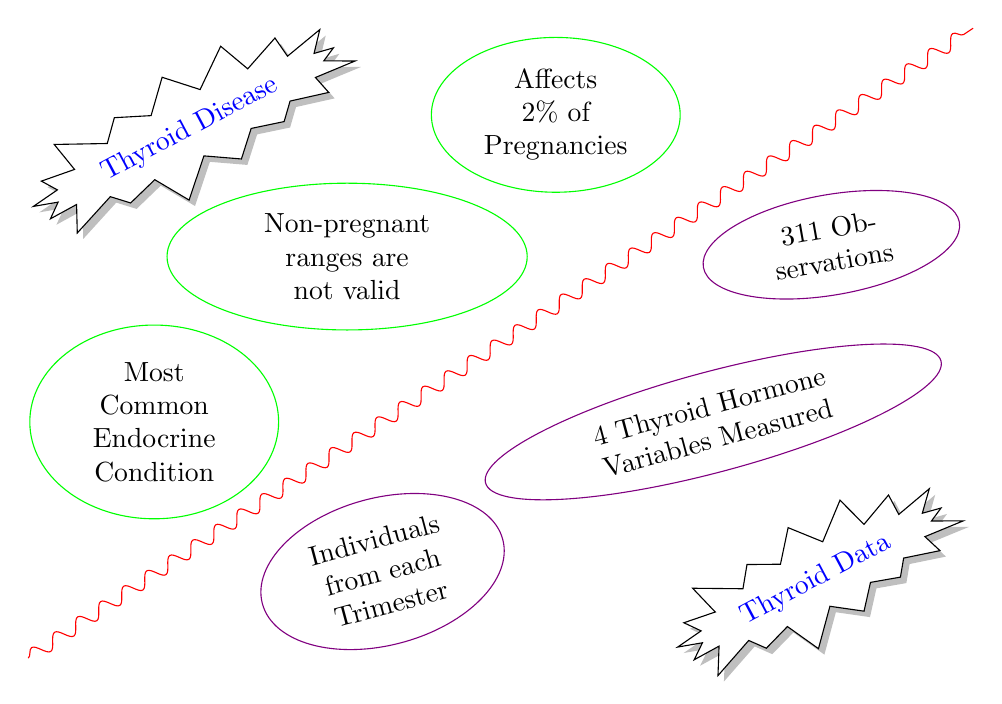
\begin{tikzpicture}
        % Line down the center of the page
        \path[decorate, decoration={snake}, draw=red] (-6,-4) -- (6,4);

        % Thyroid Disease TextBox
        \node[starburst,drop shadow,fill=white,text=blue,rotate=28,draw] at (-3.95,2.72){Thyroid Disease};

        % Thyroid Data TextBox
        \node[starburst,drop shadow,fill=white,text=blue,rotate=28,draw] at (4,-3){Thyroid Data};

        % Elements for Thyroid Data half
        \node[ellipse, text width=2.1cm,rotate=10, text centered, draw=violet] at (4.2,1.25) {311 Observations};
        \node[ellipse,rotate=15,draw=violet,text centered, text width=2cm] at (-1.5,-2.9) {Individuals from each Trimester};
        \node[ellipse, draw=violet, text centered, text width=4cm, rotate=15] at (2.7,-1) {4 Thyroid Hormone Variables Measured};

        % Elements for Thyroid Disease half
        \node[ellipse, text width=2cm, text centered, draw=green] at (0.7,2.9) {Affects 2\% of Pregnancies};
        \node[ellipse, text width=3cm, text centered, draw=green] at (-1.95,1.1) {Non-pregnant ranges are not valid};
        \node[ellipse, text width=2cm, text centered, draw=green] at (-4.4,-1) {Most Common Endocrine Condition};
    \end{tikzpicture}
    \end{figure}
}
\end{frame}
\section{Existing Methods}
\begin{frame}
\begin{figure}
    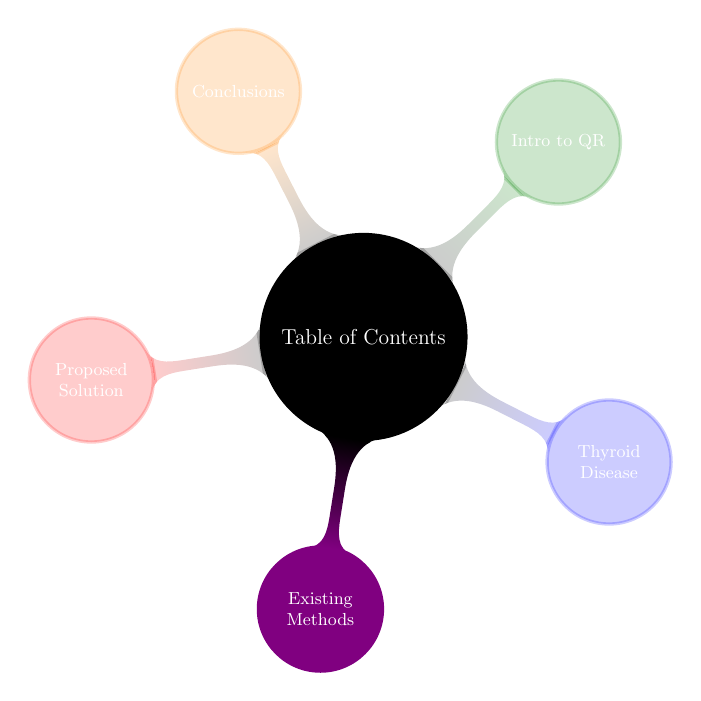
\begin{tikzpicture}[scale=0.7]
        \path[mindmap,concept color=black,text=white]
            node[concept,scale=0.65] {Table of Contents}
            [clockwise from=45]
                child[concept color=green!50!black,opacity=0.2, grow=45] {node[concept,scale=0.7,opacity=0.2,text opacity=1] {Intro to QR}}
                child[concept color=blue,opacity=0.2, grow=-27] {node[concept,scale=0.7,opacity=0.2,text opacity=1] {Thyroid Disease}}
                child[concept color=violet, grow=-99] {node[concept,scale=0.7] {Existing Methods} }
                child[concept color=red,opacity=0.2, grow=-171] {node[concept,scale=0.7,opacity=0.2,text opacity=1] {Proposed Solution}}
                child[concept color=orange,opacity=0.2, grow=117] {node[concept,scale=0.7,opacity=0.2,text opacity=1] {Conclusions} }
                ;
    \end{tikzpicture}
\end{figure}
\end{frame}

\subsection{Theory}
\begin{frame}
For each given quantile of interest, the quantile coefficients are estimated by the objective function
$$\hat{\beta}=\argmin_{\beta\in\Re^{p}}\sum\rho_{\tau}(y_{i}-x'\beta)$$

where $\rho_{\tau}$ is a check function
\vspace{6mm}

Estimating the quantiles independently of one another results in \textbf{Crossing Quantiles} - shown in the next slide
\end{frame}

\subsection{Application}
\begin{frame}
\only<1,2,3>{
\center{\textbf{\underline{Crossing Quantiles} - this shouldn't be happening!}}
    \only<1>{
        \begin{figure}
            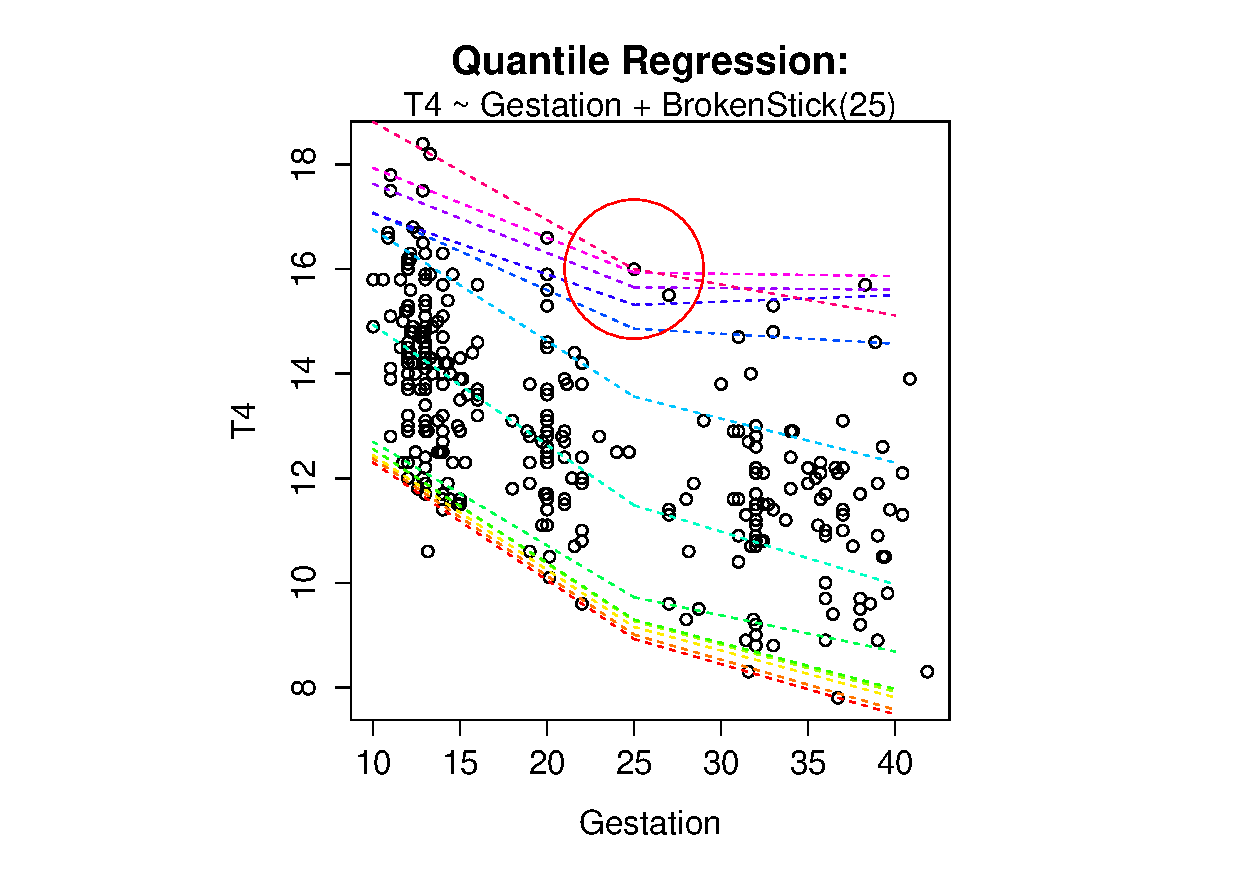
\includegraphics[width=10.5cm]{T4Circles.pdf}
        \end{figure}
    }
    \only<2>{
        \begin{figure}
            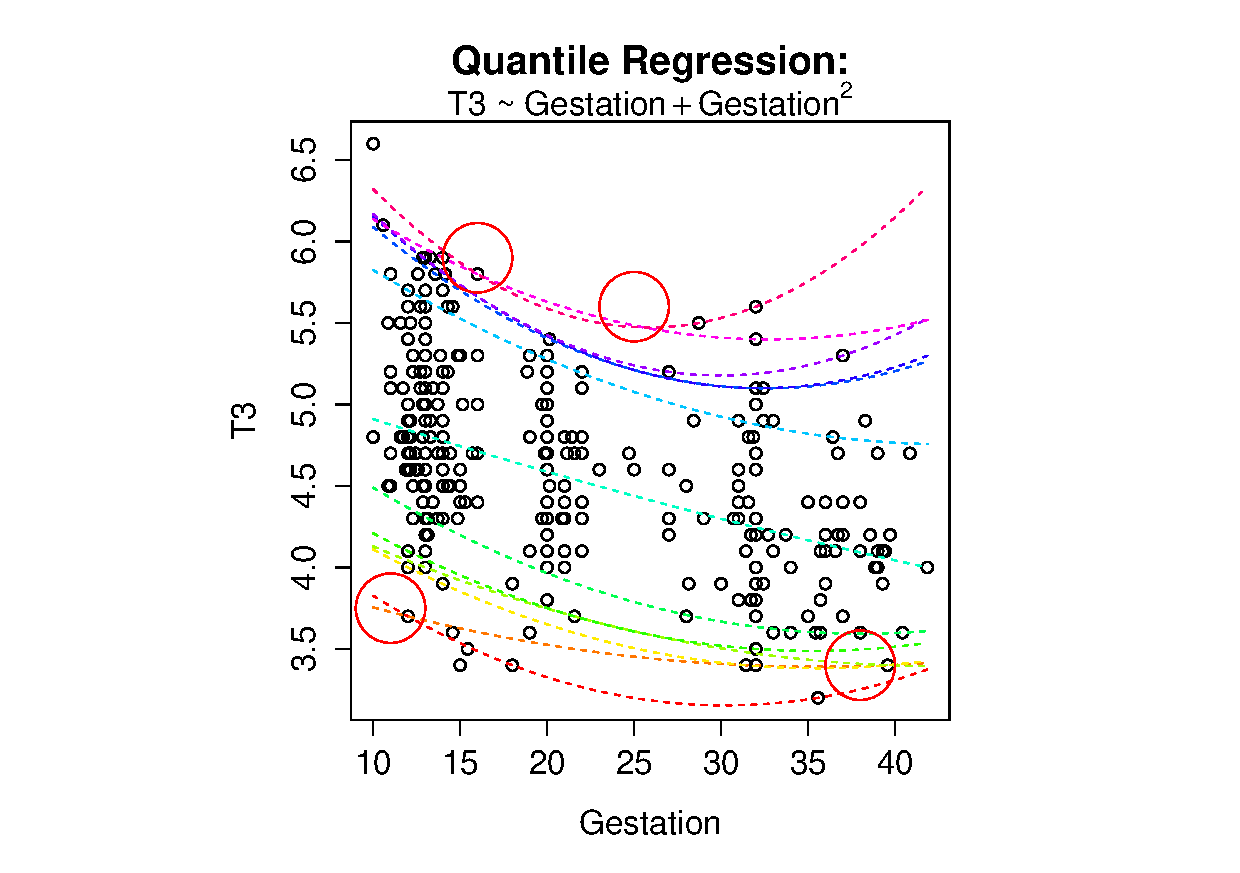
\includegraphics[width=10.5cm]{T3Circles.pdf}
        \end{figure}
    }
    \only<3>{
        \begin{figure}
            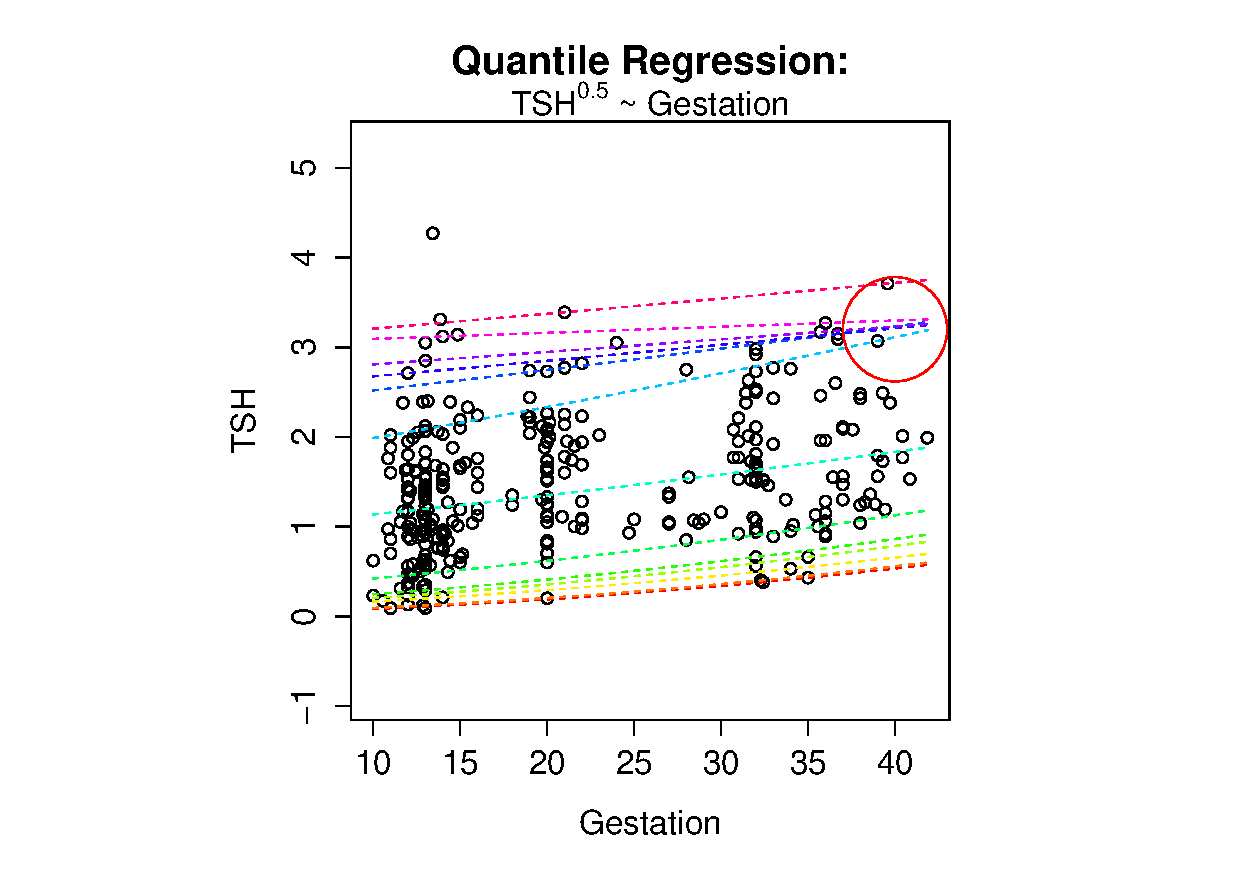
\includegraphics[width=10.5cm]{TSHCircles.pdf}
        \end{figure}
    }
}
\end{frame}

\section{Proposed Solution} % Chapter 4
\begin{frame}
\begin{figure}
    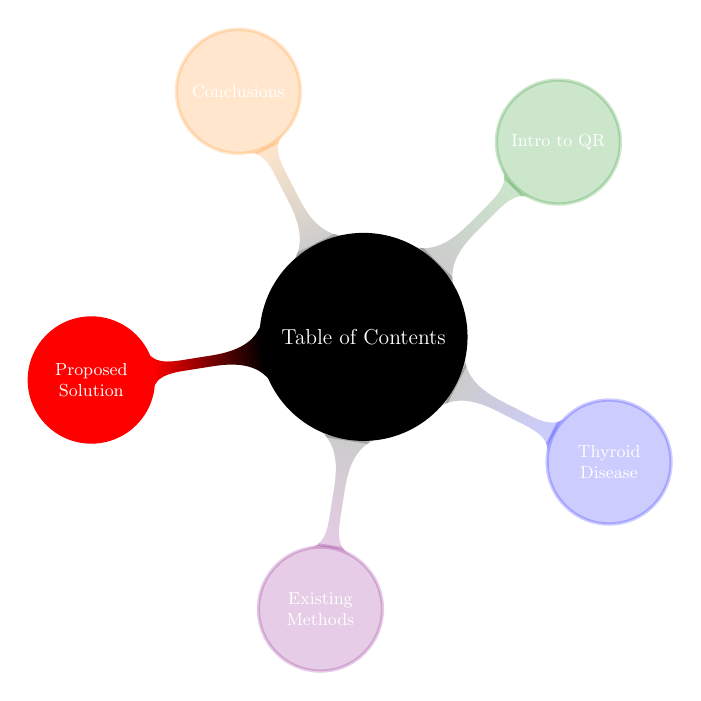
\begin{tikzpicture}[scale=0.7]
        \path[mindmap,concept color=black,text=white]
            node[concept,scale=0.65] {Table of Contents}
            [clockwise from=45]
                child[concept color=green!50!black,opacity=0.2, grow=45] {node[concept,scale=0.7,opacity=0.2,text opacity=1] {Intro to QR}}
                child[concept color=blue,opacity=0.2, grow=-27] {node[concept,scale=0.7,opacity=0.2,text opacity=1] {Thyroid Disease}}
                child[concept color=violet,opacity=0.2, grow=-99] {node[concept,scale=0.7,opacity=0.2,text opacity=1] {Existing Methods} }
                child[concept color=red, grow=-171] {node[concept,scale=0.7] {Proposed Solution}}
                child[concept color=orange,opacity=0.2,grow=117] {node[concept,scale=0.7,opacity=0.2,text opacity=1] {Conclusions} }
                ;
    \end{tikzpicture}
\end{figure}
\end{frame}

\subsection{Theory}
\begin{frame}
The objective function defined in my proposed solution is exactly the same as was previous but with additional constraints as follows:
$$\hat{\beta}=\argmin_{\beta\in\Re^{p}}\sum\rho_{\tau}(y_{i}-x'\beta)$$
\vspace{2mm}

\[\text{subject to} \;
    \begin{cases}
        \;-\hat{\beta}_{(\tau_{i})}\geq-\hat{\beta}_{(\tau_{i+1})}+\epsilon,& \text{if } 0<\tau<0.5, \\
        \;\text{no constraints},& \text{if } \tau=0.5,\\
        \;\hat{\beta}_{(\tau_{i})}\geq\hat{\beta}_{(\tau_{i-1})}+\epsilon,& \text{if } 0.5<\tau<1
    \end{cases}
\]
\vspace{6mm}

\center{This removes the issue of \textbf{Crossing Quantiles}}

\end{frame}
\begin{frame}
\begin{figure}\centering
    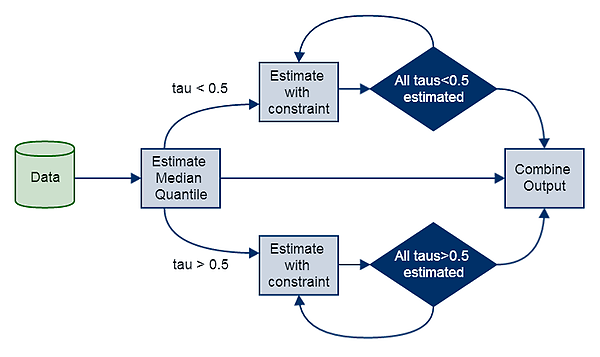
\includegraphics[width=12cm, height=8cm]{ProcessFlow.png}
\end{figure}
\end{frame}
\subsection{Application}
\begin{frame}
\only<1,3,5>{
\center{\textbf{Existing R Implementation}}
    \only<1>{
        \begin{figure}
            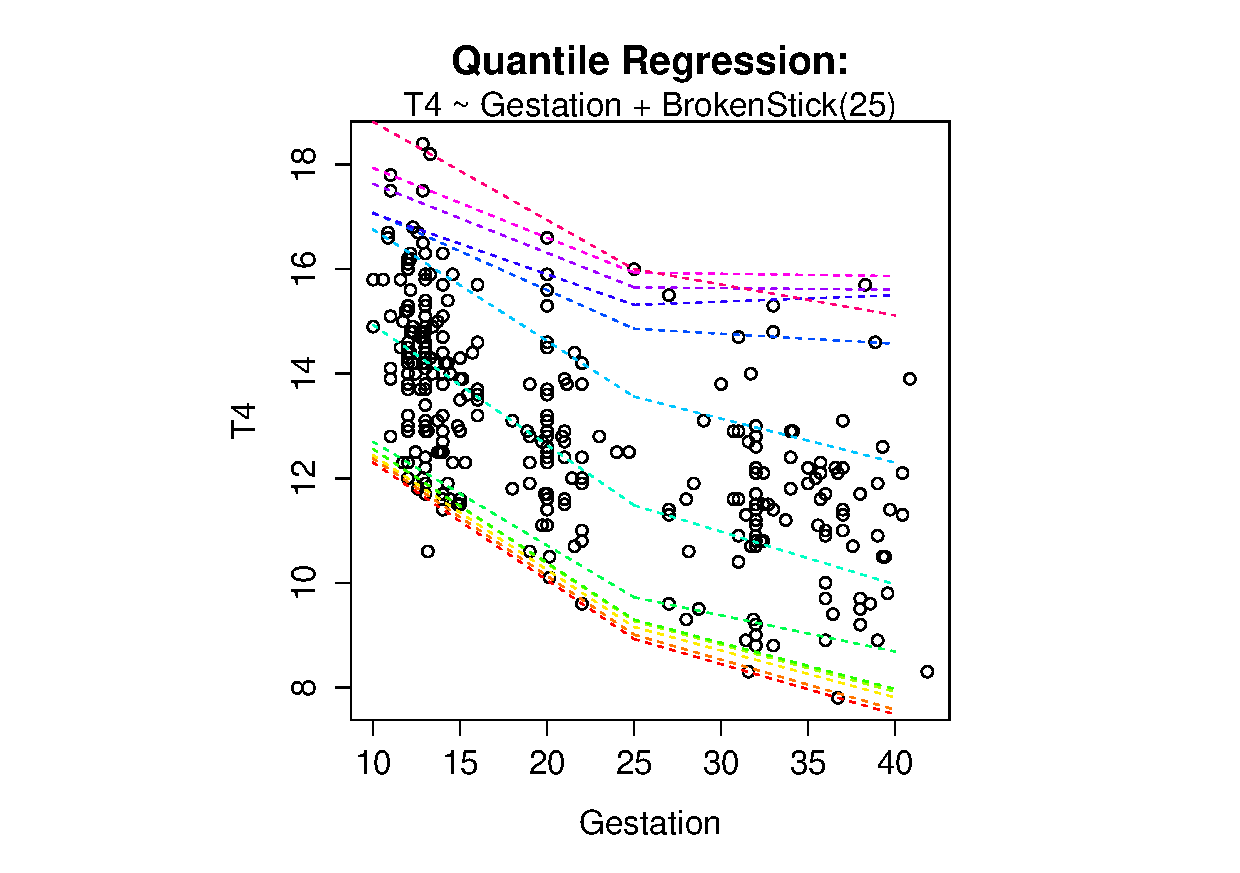
\includegraphics[width=10.5cm]{T4NoCircles.pdf}
        \end{figure}
    }
    \only<3>{
        \begin{figure}
            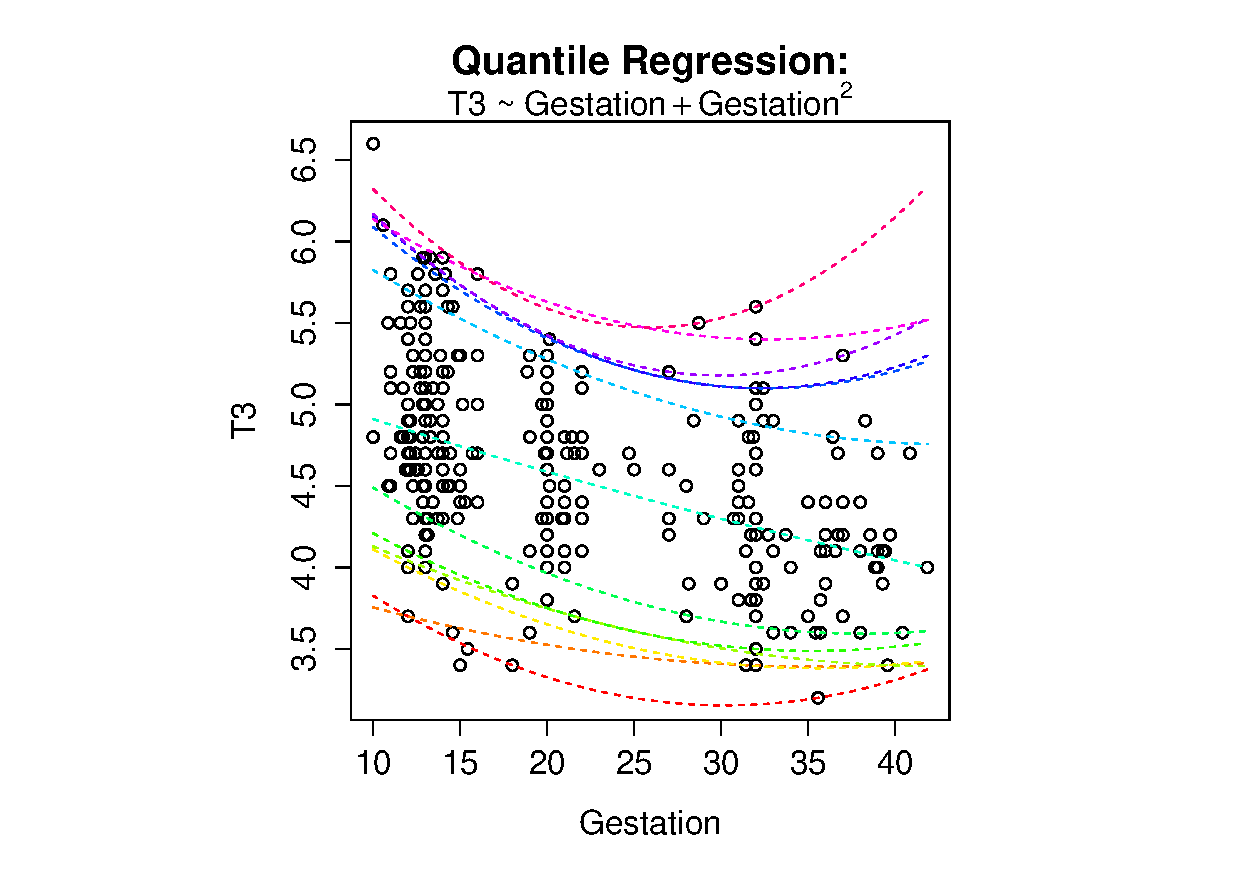
\includegraphics[width=10.5cm]{T3NoCircles.pdf}
        \end{figure}
    }
    \only<5>{
        \begin{figure}
            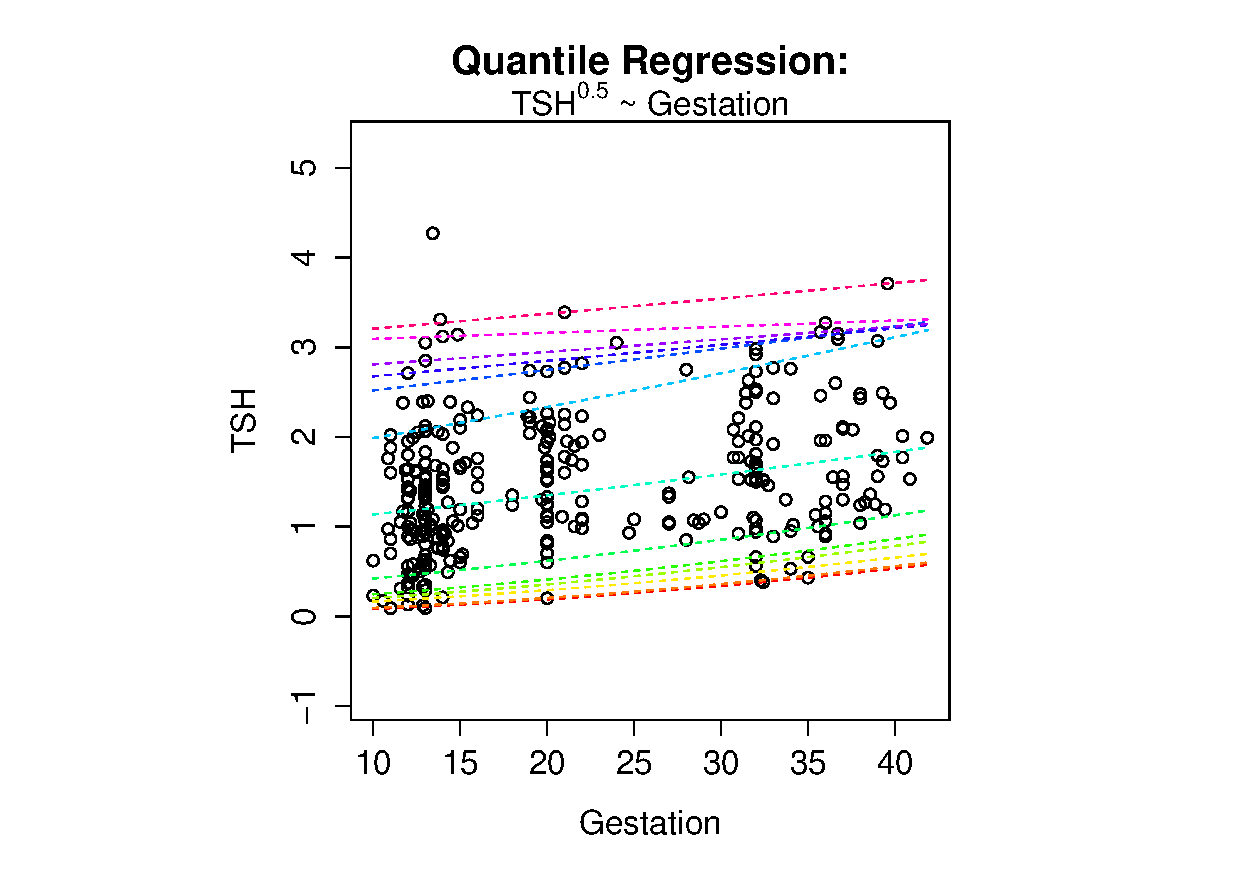
\includegraphics[width=10.5cm]{TSHNoCircles.pdf}
        \end{figure}
    }
}

\only<2,4,6>{
\center{\textbf{\underline{Non-Crossing Quantiles} - Proposed Solution}}
    \only<2>{
        \begin{figure}
            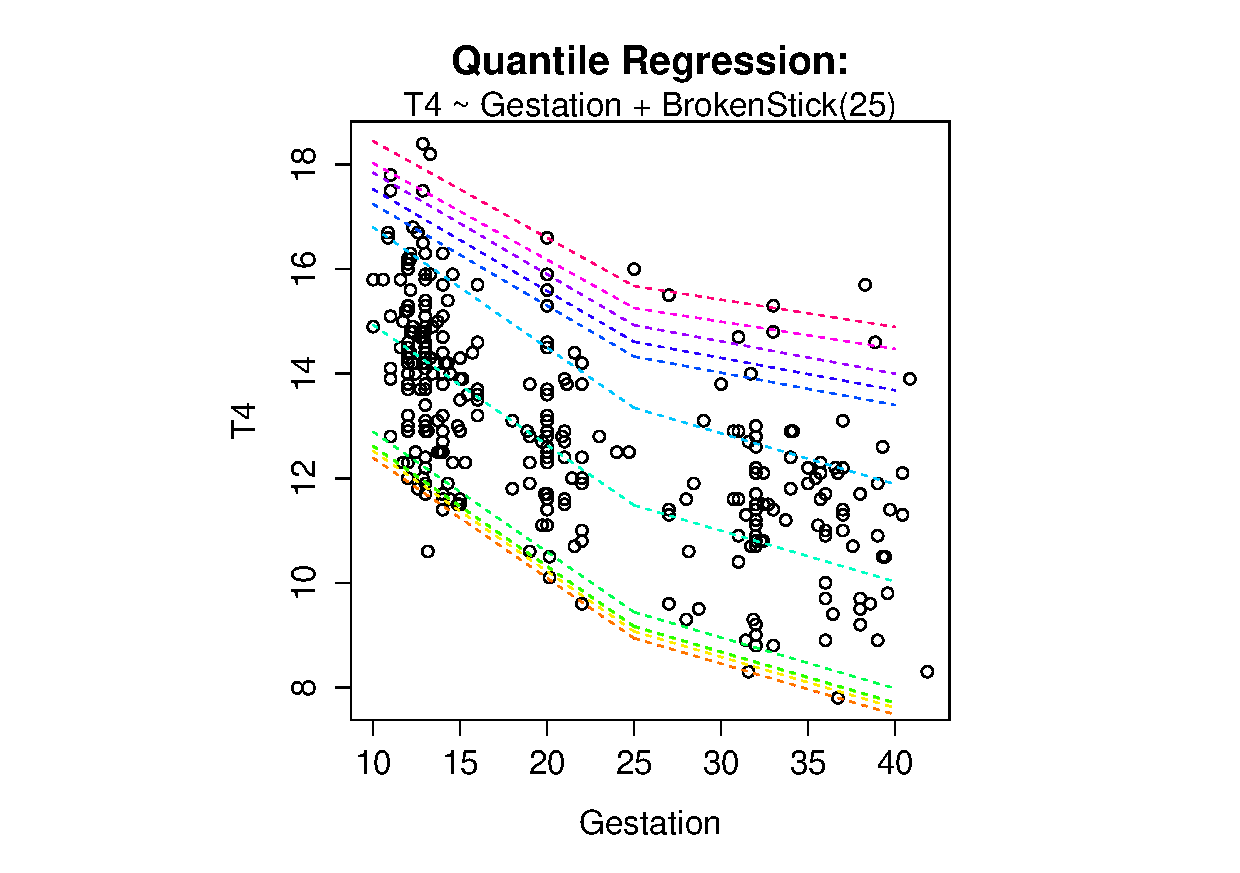
\includegraphics[width=10.5cm]{T4NonCrossing.pdf}
        \end{figure}
    }
    \only<4>{
        \begin{figure}
            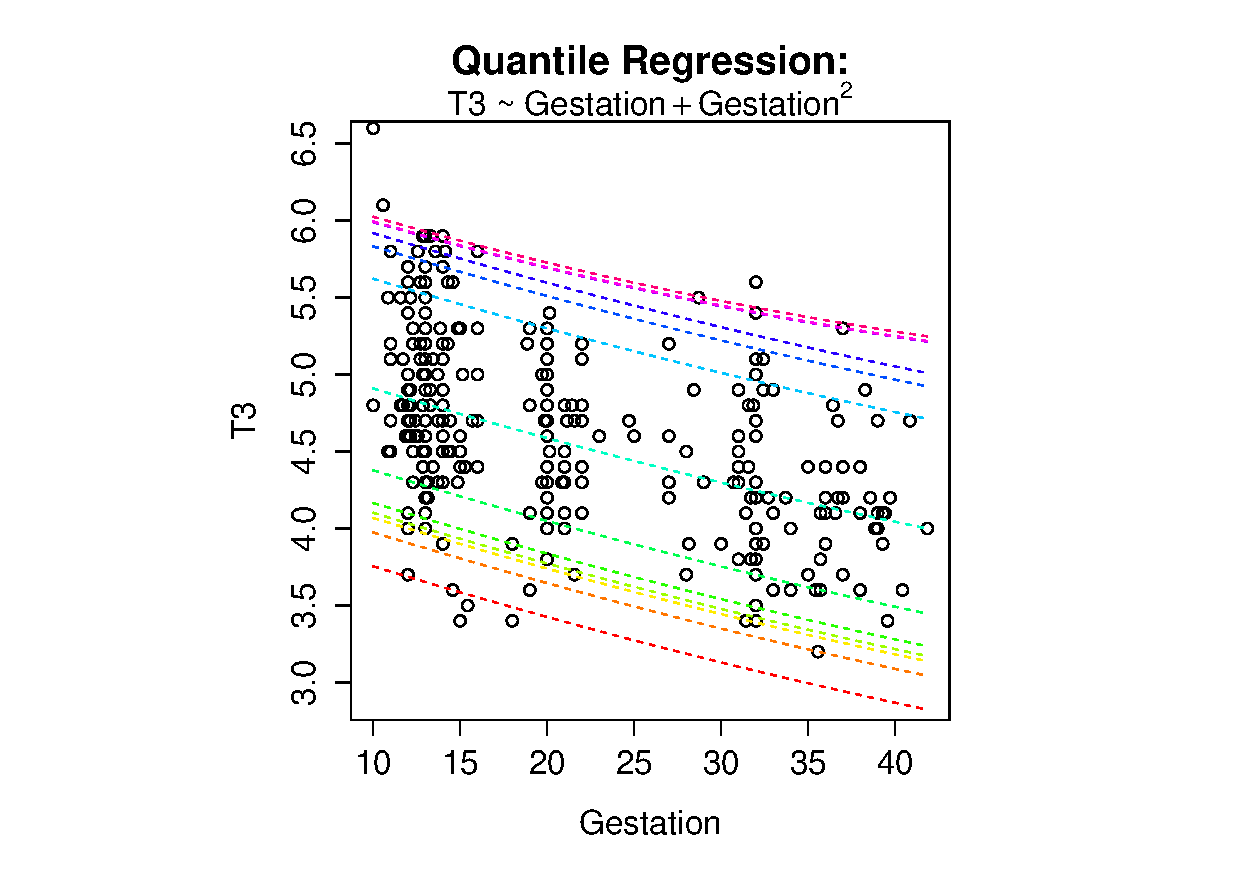
\includegraphics[width=10.5cm]{T3NonCrossing.pdf}
        \end{figure}
    }
    \only<6>{
        \begin{figure}
            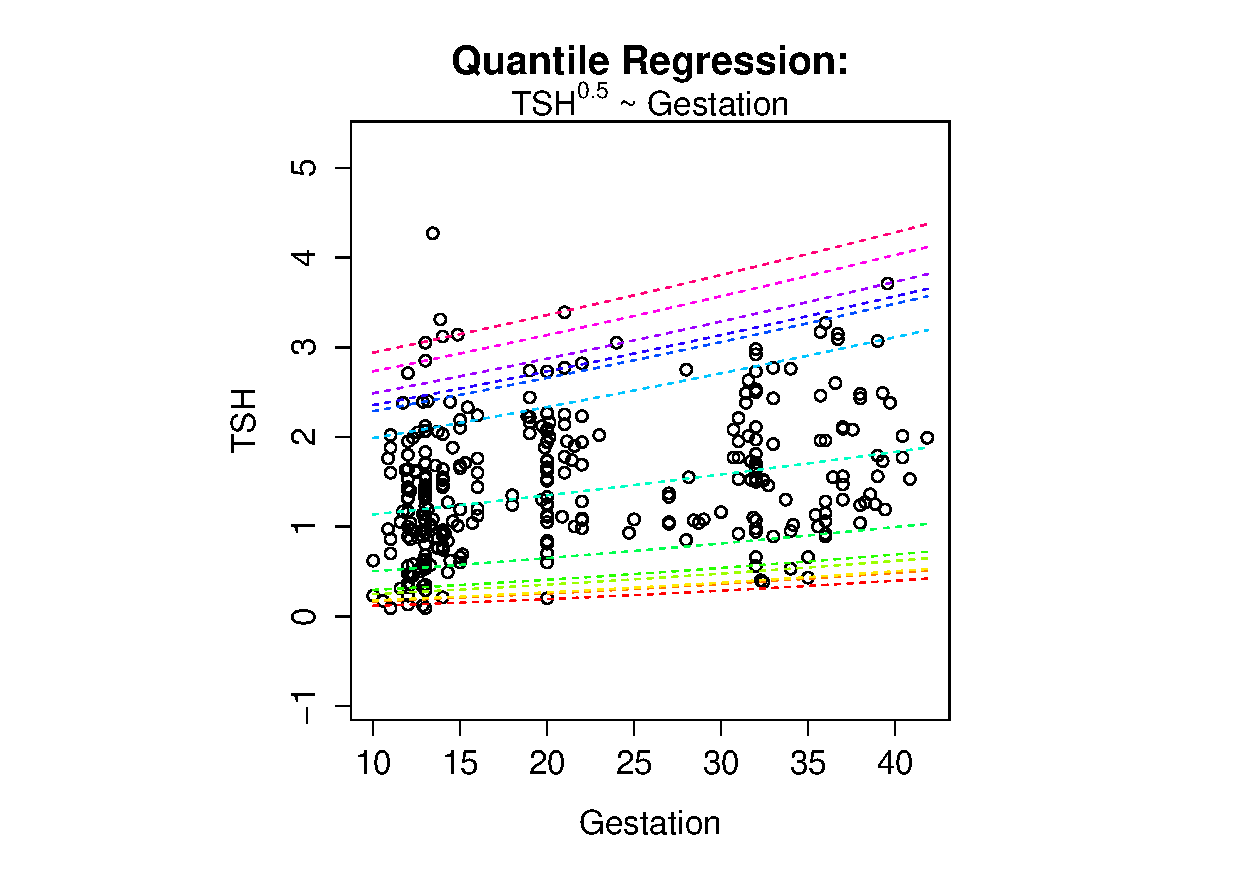
\includegraphics[width=10.5cm]{TSHNonCrossing.pdf}
        \end{figure}
    }
}
\end{frame}

\section{Conclusions} % Overall project conclusions
\begin{frame}
\begin{figure}
    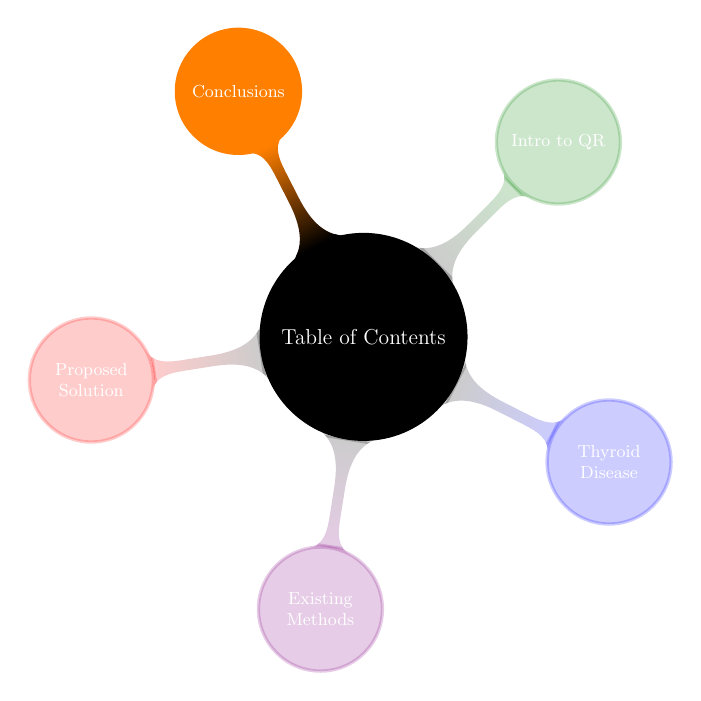
\begin{tikzpicture}[scale=0.7]
        \path[mindmap,concept color=black,text=white]
            node[concept,scale=0.65] {Table of Contents}
            [clockwise from=45]
                child[concept color=green!50!black,opacity=0.2,grow=45] {node[concept,scale=0.7,opacity=0.2,text opacity=1] {Intro to QR}}
                child[concept color=blue,opacity=0.2,grow=-27] {node[concept,scale=0.7,opacity=0.2,text opacity=1] {Thyroid Disease}}
                child[concept color=violet,opacity=0.2,grow=-99] {node[concept,scale=0.7,opacity=0.2,text opacity=1] {Existing Methods} }
                child[concept color=red,opacity=0.2,grow=-171] {node[concept,scale=0.7,opacity=0.2,text opacity=1] {Proposed Solution}}
                child[concept color=orange,grow=117] {node[concept,scale=0.7] {Conclusions} };
    \end{tikzpicture}
\end{figure}
\end{frame}

\begin{frame}
\uncover<1->{
    \textbf{Advantages}
    \vspace{2mm}
    \begin{itemize}
        \item Removes issue of crossing quantiles
        \vspace{2mm}
        \item The quantile profiles are consistent throughout the data
        \vspace{2mm}
        \item Computational effort is similar to that of existing methods
        \vspace{2mm}
        \item Easy to implement
    \end{itemize}
}
\vspace{4mm}

\uncover<2->{
    \textbf{Disadvantages}
    \vspace{2mm}
    \begin{itemize}
        \item Have not tested on simulated data
        \vspace{2mm}
        \item Have not tested on large data sets
    \end{itemize}
}
\end{frame}
\section{Q\&A} %Q&A Section
\begin{frame}
 \begin{center}
    \begin{figure}
        
\includegraphics[width=10cm]{Q&A.jpg}
    \end{figure}
    \Large{\textbf{Thanks for listening!}}
 \end{center}
\end{frame}
\end{document} 